


\documentclass[12pt,a4paper]{article}

\usepackage[T1]{fontenc}
\usepackage[utf8]{inputenc}
\usepackage{lmodern}
\usepackage{microtype}
\usepackage[a4paper,margin=2.5cm]{geometry}
\usepackage{amsmath,amssymb}
\usepackage{array,booktabs}
\usepackage{xcolor}
\usepackage{setspace}
\usepackage[hidelinks]{hyperref}
\usepackage{tikz}
\usetikzlibrary{arrows.meta,positioning}
\usepackage{graphicx}

\setlength{\parindent}{1.3em}
\setlength{\parskip}{0pt}
\setlength{\emergencystretch}{2em}
\newcolumntype{P}[1]{>{\raggedright\arraybackslash}p{#1}}

\begin{document}
	
	\begin{center}
		{\Large\bfseries Physics-guided search and graph learning for conductive-
			particle allocation in a polydisperse packed bed\par}
		\vspace{1.0em}
		{\normalsize Ali Khalifa and ......\par}
		\vspace{0.45em}
		{\small Technical University of Munich, Freising, Germany.}
	\end{center}
	
	\vspace{1em}
	\setstretch{1.35}
	
	\begin{abstract}
		A packed thermal store containing a limited amount of highly conductive
		material can perform differently depending on where that material is placed.
		This study isolates that placement effect while keeping packing geometry,
		porosity, particle-size distribution and conductive-material volume fixed.
		Ten independent 500-particle packings with three diameter classes
		(1.5, 2.0 and 2.5~mm) were generated by the discrete-element method at a
		nominal porosity of 0.38. A verified steady contact-network solver evaluated
		random placement, contact-degree and baseline heat-path rankings, and a
		fixed-budget same-size swap search. The best searched assignments increased
		effective conductivity by $56.3\pm4.1$\% relative to random placement.
		A graph neural network (GNN) was then trained to imitate the recurring
		selections of five independent search restarts and was tested by
		leave-one-packing-out cross-validation. A non-graph multilayer perceptron
		(MLP) received exactly the same particle features. On unseen packings, the MLP
		and GNN obtained $k_{\mathrm{eff}}=0.13137\pm0.00583$ and
		$0.14189\pm0.00731$~W\,m$^{-1}$\,K$^{-1}$, respectively, compared with
		$0.12208\pm0.00467$ for the transparent heat-path rule. The GNN exceeded both
		baselines in all ten held-out packings and recovered
		$50.7\pm7.7$\% of the gain between random placement and the best searched
		assignment; the MLP recovered $33.6\pm4.3$\%. Once trained, the GNN required
		one homogeneous feature solve, approximately 4~ms of CPU inference and one
		verification solve, whereas teacher generation used about 14829 distinct
		thermal evaluations per packing. Mechanism analysis showed that
		the improvement arises from cooperative, vertically useful conductive paths
		rather than local coordination alone. The results establish graph learning as
		a useful fast allocation model for unseen realizations of the investigated
		stationary, contact-dominated bed. Fluid convection, radiation and transfer to
		other packing specifications remain outside the present scope.
	\end{abstract}
	
	\noindent\textbf{Keywords:} packed-bed thermal energy storage; granular heat
	conduction; discrete-element method; graph neural network; material allocation;
	inverse design
	
	\section{Introduction}
	
	Heat transfer through a packed bed depends on particle conductivity, particle
	size, porosity, contact area and the organization of the contact network.
	Classical theory and thermal discrete-element models describe how these factors
	determine heat flow through a specified granular structure
	\cite{Batchelor1977,Vargas2001,Kiani2019,Joulin2020}. Most such calculations are
	forward problems: the packing and material distribution are prescribed, and
	the resulting temperature field or effective conductivity is calculated.
	
	Many engineering beds, however, contain a limited amount of an expensive or
	specialized conductive phase. In that situation, the practical question is not
	only how much conductive material is present, but where it should be placed.
	Random mixing can put conductive particles in regions that carry little net
	heat. Selecting particles with many contacts may also be inefficient, because a
	highly connected particle can lie on a side branch rather than on a route that
	links the hot and cold boundaries.
	
	Inverse design on graph-structured materials has been considered for
	architected lattices \cite{Dold2023}. A packed bed creates a different problem:
	the graph is not freely drawn or deformed, but is the mechanically admissible
	contact network produced by particle packing. The geometry remains fixed and
	only the particle material labels are changed. This gives a controlled question:
	
	\begin{quote}
		At fixed porosity, particle-size distribution and conductive-material volume,
		can the effective conductivity of a packed bed be increased substantially by
		placing conductive particles according to the global heat-transfer network?
	\end{quote}
	
	We address this question using ten independent DEM packings, a verified steady
	thermal contact network and four increasingly informed allocation strategies.
	We then ask whether a learned model can transfer the allocation rule to a
	previously unseen packing without performing thousands of trial thermal solves.
	An edge-aware GNN is compared with a non-graph MLP supplied with exactly the
	same particle features. This comparison separates the value of contact-network
	message passing from the value of the input features themselves.
	
	Figure~\ref{fig:problem} summarizes the physical problem. DEM first fixes the
	particle positions and contacts. The material budget is then allocated without
	moving any particle or changing the packing porosity and particle-size
	distribution. The present paper considers heat conduction through solid
	contacts only; stagnant-fluid conduction is reserved for a later, separately
	validated extension. The investigated millimetre-scale spheres represent the
	lower end of particle sizes used in solid-particle thermal storage and provide a
	controlled model bed rather than a calibrated representation of one particular
	commercial storage material \cite{Zeng2025,Boribayeva2024}.
	
\begin{figure}[!htbp]
	\centering
	\resizebox{0.85\textwidth}{!}{%
		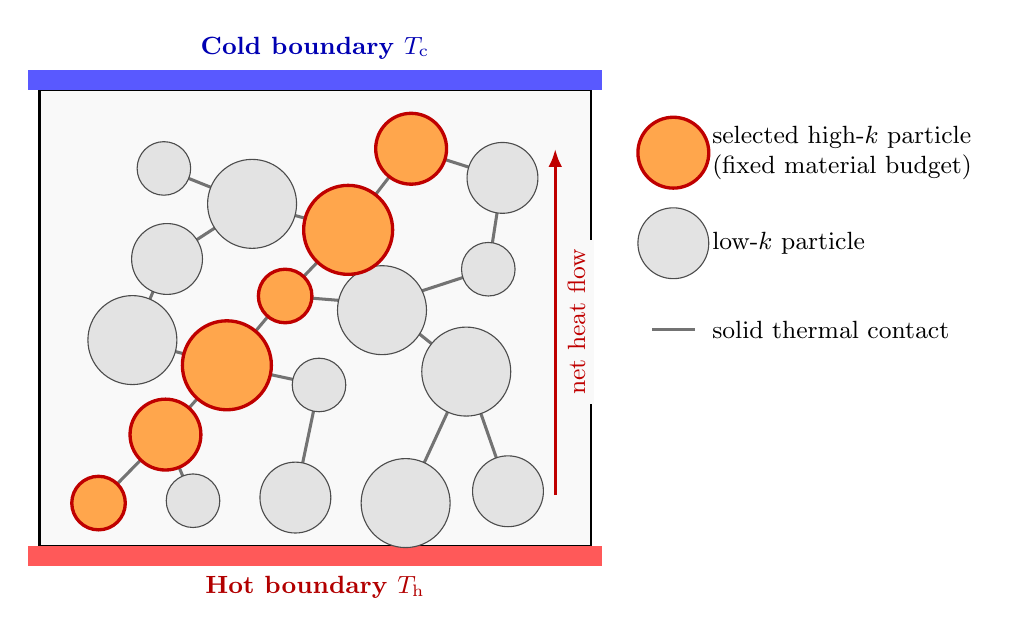
\begin{tikzpicture}[
			% Low-conductivity particles
			particleSmall/.style={
				circle,
				draw=black!70,
				fill=gray!22,
				minimum size=6.8mm,
				inner sep=0pt
			},
			particleMedium/.style={
				circle,
				draw=black!70,
				fill=gray!22,
				minimum size=9.0mm,
				inner sep=0pt
			},
			particleLarge/.style={
				circle,
				draw=black!70,
				fill=gray!22,
				minimum size=11.3mm,
				inner sep=0pt
			},
			% High-conductivity particles
			conductiveSmall/.style={
				circle,
				draw=red!75!black,
				very thick,
				fill=orange!70,
				minimum size=6.8mm,
				inner sep=0pt
			},
			conductiveMedium/.style={
				circle,
				draw=red!75!black,
				very thick,
				fill=orange!70,
				minimum size=9.0mm,
				inner sep=0pt
			},
			conductiveLarge/.style={
				circle,
				draw=red!75!black,
				very thick,
				fill=orange!70,
				minimum size=11.3mm,
				inner sep=0pt
			},
			contact/.style={
				draw=black!55,
				line width=1.1pt
			},
			heat/.style={
				-{Latex[length=2.3mm]},
				red!75!black,
				very thick
			},
			labelbox/.style={
				align=left,
				font=\small
			}
			]
			
			% Packed-bed domain and thermal boundaries
			\fill[gray!5] (0,0) rectangle (7,5.8);
			\draw[thick] (0,0) rectangle (7,5.8);
			
			\fill[red!65] (-0.15,-0.25) rectangle (7.15,0);
			\fill[blue!65] (-0.15,5.8) rectangle (7.15,6.05);
			
			\node[
			font=\small\bfseries,
			red!70!black
			] at (3.5,-0.52)
			{Hot boundary $T_{\mathrm h}$};
			
			\node[
			font=\small\bfseries,
			blue!70!black
			] at (3.5,6.33)
			{Cold boundary $T_{\mathrm c}$};
			
			% Particle-contact network
			\draw[contact]
			(0.75,0.55)--(1.60,1.42)--(2.38,2.30)--
			(3.12,3.18)--(3.92,4.02)--(4.72,5.05);
			
			\draw[contact] (1.95,0.58)--(1.60,1.42);
			\draw[contact] (2.38,2.30)--(1.18,2.62);
			\draw[contact] (2.38,2.30)--(3.55,2.05);
			\draw[contact] (3.12,3.18)--(4.35,3.08);
			\draw[contact] (3.92,4.02)--(2.70,4.35);
			\draw[contact] (4.72,5.05)--(5.88,4.68);
			
			% Additional low-conductivity contacts
			\draw[contact] (3.25,0.62)--(3.55,2.05);
			\draw[contact] (4.65,0.55)--(5.42,2.22);
			\draw[contact] (5.95,0.70)--(5.42,2.22);
			\draw[contact] (1.18,2.62)--(1.62,3.65);
			\draw[contact] (1.62,3.65)--(2.70,4.35);
			\draw[contact] (4.35,3.08)--(5.42,2.22);
			\draw[contact] (4.35,3.08)--(5.70,3.52);
			\draw[contact] (5.70,3.52)--(5.88,4.68);
			\draw[contact] (2.70,4.35)--(1.58,4.80);
			
			% Low-conductivity particles: three size classes
			\node[particleSmall]  at (1.95,0.58) {};
			\node[particleMedium] at (3.25,0.62) {};
			\node[particleLarge]  at (4.65,0.55) {};
			\node[particleMedium] at (5.95,0.70) {};
			
			\node[particleLarge]  at (1.18,2.62) {};
			\node[particleSmall]  at (3.55,2.05) {};
			\node[particleLarge]  at (5.42,2.22) {};
			
			\node[particleMedium] at (1.62,3.65) {};
			\node[particleLarge]  at (4.35,3.0) {};
			\node[particleSmall]  at (5.70,3.52) {};
			
			\node[particleLarge]  at (2.70,4.35) {};
			\node[particleSmall]  at (1.58,4.80) {};
			\node[particleMedium] at (5.88,4.68) {};
			
			% Selected high-conductivity particles
			\node[conductiveSmall]  at (0.75,0.55) {};
			\node[conductiveMedium] at (1.60,1.42) {};
			\node[conductiveLarge]  at (2.38,2.30) {};
			\node[conductiveSmall]  at (3.12,3.18) {};
			\node[conductiveLarge]  at (3.92,4.02) {};
			\node[conductiveMedium] at (4.72,5.05) {};
			
			% Net heat-flow direction
			\draw[heat] (6.55,0.65)--(6.55,5.05);
			
			\node[
			font=\small,
			rotate=90,
			red!75!black,
			fill=gray!5
			] at (6.82,2.85)
			{net heat flow};
			
			% Material legend
			\node[conductiveMedium] at (8.05,5.00) {};
			
			\node[
			labelbox,
			anchor=west
			] at (8.42,5.00)
			{selected high-$k$ particle\\
				(fixed material budget)};
			
			\node[particleMedium] at (8.05,3.85) {};
			
			\node[
			labelbox,
			anchor=west
			] at (8.42,3.85)
			{low-$k$ particle};
			
			% Contact legend
			\draw[contact] (7.78,2.75)--(8.32,2.75);
			
			\node[
			labelbox,
			anchor=west
			] at (8.42,2.75)
			{solid thermal contact};
			
			% Particle-size legend
%			\node[
%			labelbox,
%			anchor=west,
%			font=\small\bfseries
%			] at (7.75,1.80)
%			{Particle-size classes:};
%			
%			\node[particleSmall] at (8.02,1.20) {};
%			\node[particleMedium] at (9.20,1.20) {};
%			\node[particleLarge] at (10.55,1.20) {};
%			
%			\node[
%			font=\scriptsize,
%			anchor=north
%			] at (8.02,0.85)
%			{$1.5$ mm};
%			
%			\node[
%			font=\scriptsize,
%			anchor=north
%			] at (9.20,0.75)
%			{$2.0$ mm};
%			
%			\node[
%			font=\scriptsize,
%			anchor=north
%			] at (10.55,0.65)
%			{$2.5$ mm};
%			
			% Fixed-geometry explanation
%			\node[
%			labelbox,
%			anchor=west,
%			text width=4.2cm
%			] at (7.78,-0.10)
%			{DEM fixes particle positions, particle sizes and contact topology.
%				Only the material labels are changed.};
%			
		\end{tikzpicture}%
	}
	
	\caption{Schematic of the inverse allocation problem for a polydisperse packed
		bed. The three illustrated particle sizes represent the simulated diameter
		classes of 1.5, 2.0 and 2.5~mm. DEM fixes the particle positions, particle-size
		distribution and contact network. A prescribed number of particles from each
		size class receives the high-conductivity material, while the packing geometry
		and total conductive-material volume remain unchanged. Heat is conducted
		through the fixed solid-contact network.}
	
	\label{fig:problem}
\end{figure}
	
	\section{Methods}
	
	\subsection{Controlled DEM packing ensemble}
	
	The packings were generated with LAMMPS (22 July 2025, Update 5) using spherical
	particles and a non-cohesive Hertz--Mindlin contact law
	\cite{CundallStrack1979,LAMMPSGranular}. Each realization contains 500 particles
	in a cubic cell of side $H=15.3706$~mm. The $x$ and $y$ directions are periodic,
	whereas flat mechanical walls at $z=0$ and $z=H$ confine the bed. Gravity was
	omitted because the purpose was to generate statistically different,
	equal-volume representative contact networks without a vertical compaction
	gradient.
	
	The number-based particle-size distribution (PSD) is 100 particles of diameter
	1.5~mm, 300 of diameter 2.0~mm and 100 of diameter 2.5~mm, corresponding to
	20/60/20\% by number. These three discrete sizes introduce controlled
	polydispersity while retaining exact size-class quotas during material
	allocation. Diameters of 1--100~mm occur across solid-particle storage concepts;
	the present 1.5--2.5~mm interval lies at the small-particle end, where large
	surface area is attractive for heat exchange but pressure drop becomes an
	important system-level constraint \cite{Zeng2025,Knoedler2019}. The selected
	density, $2500$~kg\,m$^{-3}$, is representative of mineral and ceramic sensible-
	heat media. These choices define a generic model system: they support a
	mechanistic investigation of contact-network allocation but are not claimed to
	reproduce one named rock, slag or ceramic.
	
	The exact undeformed solid volume,
	$V_s=\sum_i\pi d_i^3/6$, was used to set the cell volume through
	$H^3=V_s/(1-\varepsilon)$ with target porosity $\varepsilon=0.38$. This value is
	consistent with a dense random sphere packing and is relevant to stationary
	packed-bed stores, in which packing fraction and particle arrangement affect
	both thermal transport and thermomechanical loading
	\cite{Knoedler2019,Garitaonandia2024}. Because the particle counts, diameters and
	cell volume are exact, all realizations have the same nominal porosity and PSD by
	construction rather than by post-hoc matching.
	
	Table~\ref{tab:demsettings} gives the mechanical and numerical parameters. The
	normal force is Hertzian, the history-dependent tangential force follows the
	Mindlin model with Coulomb limit, and Tsuji damping uses the specified
	restitution coefficient. The same law is used at the two vertical walls. The
	Young modulus of 50~MPa is deliberately softened relative to many rocks and
	ceramics to make quasistatic packing generation affordable. It is therefore a
	numerical packing parameter, not a calibrated storage-material property. This
	qualification matters because the subsequent thermal contact radius is computed
	from the final DEM overlap; sensitivity to stiffness is accordingly retained as
	a limitation.
	
	\begin{table}[!htbp]
		\centering
		\caption{DEM packing-generation parameters used for every realization.}
		\label{tab:demsettings}
		\small
		\begin{tabular}{P{5.6cm}P{6.3cm}}
			\toprule
			\textbf{Quantity} & \textbf{Value or model} \\
			\midrule
			Particle count and diameters & $500$; 100 at 1.5~mm, 300 at 2.0~mm, 100 at 2.5~mm \\
			Density & 2500~kg\,m$^{-3}$ \\
			Target porosity and cell side & 0.38; 15.3706~mm \\
			Boundary conditions & periodic $x,y$; fixed flat walls at $z=0,H$; no gravity \\
			Normal contact & Hertz material model; $E=5.0\times10^7$~Pa, $\nu=0.25$ \\
			Tangential contact & Mindlin history with rescaling; friction coefficient $\mu=0.50$ \\
			Collision damping & Tsuji model; restitution coefficient $e=0.30$; tangential damping multiplier 1.0 \\
			Time integration & explicit velocity-Verlet for translating and rotating spheres (\texttt{nve/sphere}) \\
			Time step & $2.0\times10^{-7}$~s \\
			Packing schedule & diameter growth: 300000 steps; final-size relaxation: 200000 steps \\
			Viscous relaxation & $10^{-3}$ during growth; $0.10$ after growth (LAMMPS SI units) \\
			\bottomrule
		\end{tabular}
	\end{table}
	
	Particle centres were initially sampled from the seed-dependent uniform random
	distribution while all diameters were reduced to 5\% of their final values. The
	three classes were expanded linearly to their prescribed diameters over 300000
	steps, followed by 200000 steps of damped relaxation at final size. Translational
	and rotational equations were advanced with the explicit velocity-Verlet scheme
	implemented by \texttt{fix nve/sphere} \cite{LAMMPSNVESphere}. The time step
	$2.0\times10^{-7}$~s is approximately 0.7\% of the estimated Rayleigh time of the
	smallest sphere for the stated softened elastic properties, providing a
	conservative resolution of the contact dynamics. Neighbour lists were checked
	every step and loss of any particle was treated as an error.
	
	Ten seeds generated ten different initial centre arrangements and hence ten
	different contact networks. Particle counts, sizes, material parameters, cell
	dimensions, growth schedule and relaxation schedule were otherwise identical.
	Final particle volumes and the 100/300/100 counts were written to a packing
	summary and checked against their requested values. The resulting graphs
	contained 1325--1382 particle--particle contacts, and every packing contained one
	large contact component connecting the lower and upper thermal walls.
	
	\subsection{Steady thermal contact network}
	
	Each particle is represented by a graph node and every DEM contact by a thermal
	edge. For an internal particle $i$, steady energy conservation is
	\begin{equation}
		\sum_{j\in\mathcal N_i}G_{ij}(T_j-T_i)=0,
		\label{eq:balance}
	\end{equation}
	where $G_{ij}$ is the contact conductance. For two particles with conductivities
	$k_i$ and $k_j$ and contact radius $a_{ij}$, the constriction model is
	\begin{equation}
		G_{ij}=\frac{2a_{ij}k_i k_j}{k_i+k_j},
		\qquad
		a_{ij}=\sqrt{R_{ij}^{*}\delta_{ij}},
		\label{eq:conductance}
	\end{equation}
	where $R_{ij}^{*}=R_iR_j/(R_i+R_j)$ and $\delta_{ij}$ is the DEM overlap. Fixed
	temperatures of 301 and 300~K were applied at the lower and upper walls. The
	effective conductivity follows from
	\begin{equation}
		k_{\mathrm{eff}}=\frac{QH}{A(T_{\mathrm h}-T_{\mathrm c})},
		\label{eq:keff}
	\end{equation}
	where $Q$ is the wall heat rate, $H$ is bed height and $A$ is cross-sectional
	area. Wall conductance uses the corresponding sphere--plane contact radius and
	an infinite wall conductivity, so the finite resistance lies on the particle
	side. The assembled balances form a sparse symmetric conductance system.
	Components connected to neither thermal wall have no unique absolute
	temperature and carry no boundary-to-boundary heat; they are identified by graph
	connectivity, omitted from the linear solve and reported separately. The
	remaining sparse linear system is solved directly in double precision. Effective
	conductivity is calculated from both wall heat rates, whose relative mismatch
	provides the energy-balance error.
	
	The present paper uses solid-contact conduction only. A preliminary stagnant-air
	gap model was tested, but its predicted conductivity depended too strongly on
	an arbitrary neighbour cutoff. Those results were therefore excluded from the
	allocation conclusions. This choice makes the present scope a stationary,
	contact-dominated bed rather than a flowing or convective system.
	
	\subsection{Fixed material budget}
	
	The low- and high-conductivity materials were assigned
	$k_{\mathrm L}=1$ and $k_{\mathrm H}=10$~W\,m$^{-1}$\,K$^{-1}$. A binary
	variable $x_i$ indicates whether particle $i$ receives the high-conductivity
	material:
	\begin{equation}
		k_i=k_{\mathrm L}+x_i(k_{\mathrm H}-k_{\mathrm L}).
	\end{equation}
	
	Because the bed is polydisperse, selecting the same total number of particles
	does not automatically select the same material volume. Every allocation was
	therefore constrained to contain 10 small, 30 medium and 10 large
	high-conductivity particles. The selected conductive-particle volume was
	$2.2514747\times10^{-7}$~m$^3$ in every calculation. This constraint preserves
	both the conductive-particle count and its size distribution.
	
	\subsection{Allocation strategies}
	
	Four strategies were compared on every fixed packing:
	
	\begin{enumerate}
		\item \textbf{Random placement:} 100 independent assignments satisfying the
		size-class quotas. Their mean and standard deviation define the undesigned
		reference.
		\item \textbf{Degree ranking:} within each size class, particles with the most
		contacts are selected first.
		\item \textbf{Heat-path ranking:} the homogeneous low-conductivity bed is
		solved first. Each particle receives the score
		\begin{equation}
			S_i=\sum_j\left|G_{ij}(T_i-T_j)\right|,
		\end{equation}
		which measures the baseline heat passing through its incident contacts. The
		highest-scoring particles are selected within each size class.
		\item \textbf{Fixed-budget same-size swap search:} the search starts from the
		better of degree and heat-path ranking. One selected and one unselected
		particle of the same size class exchange their material labels. The proposal
		is retained only when it increases $k_{\mathrm{eff}}$. Each of five independent
		restarts is limited to exactly 3000 proposed swaps.
	\end{enumerate}
	Here, ``same-size swap'' describes the search move, whereas ``fixed budget''
	describes its stopping rule; together they define one algorithm, not two
	different methods. Restricting each exchange to one size class preserves the
	number, size distribution and total volume of high-conductivity particles.
	Similar exchange strategies are widely used in
	combinatorial optimization
	\cite{KernighanLin1970,Maringer2003}, although our implementation is adapted
	specifically to the packed-bed thermal problem. Because only a fixed number of
	proposals is tested, the method identifies a good allocation but does not
	guarantee the global optimum. We report both the mean final result across the
	five restarts and the best final result among them. Performance is evaluated relative to the mean
	result obtained from random allocations in the same packing:
	\begin{equation}
		I=100\frac{k_{\mathrm{eff}}-\overline{k}_{\mathrm{eff,random}}}
		{\overline{k}_{\mathrm{eff,random}}}\;[\%].
		\label{eq:improvement}
	\end{equation}
	
	\subsection{Graph-learning allocation models}

	The fixed-budget same-size swap search provides high-quality assignments but requires repeated thermal
	solutions. We therefore tested whether a supervised model could learn a fast
	particle-ranking rule and transfer it to a packing not used during training. One
	graph was constructed for each DEM realization. Nodes are particles; each
	undirected DEM contact is stored as two directed edges so that messages can pass
	in both directions.

	\paragraph{Inputs and target.}
	Each node has eight features: diameter divided by the reference diameter,
	normalized vertical position, contact degree, hot-wall-contact flag,
	cold-wall-contact flag, membership in a thermally wall-anchored component,
	normalized temperature in the homogeneous $k_{\mathrm L}$ solution, and the
	normalized baseline heat-path score. Each directed edge has six features:
	normalized contact radius; the three normalized minimum-image components
	$\Delta x$, $\Delta y$ and $\Delta z$; absolute vertical alignment
	$|\Delta z|/d_{ij}$; and normalized absolute contact heat rate in the
	homogeneous solution. All inputs are available before the high-conductivity
	material is allocated.

	The teaching signal is obtained from the five final same-class swap-search
	restarts for the corresponding packing. For particle $i$, the soft target
	$y_i\in\{0,0.2,\ldots,1\}$ is the fraction of restarts that selected it. This
	captures recurring choices instead of forcing the model to copy only one
	stochastic best assignment. Binary membership of the best restart is retained
	only for Jaccard evaluation and is not an input. The soft targets sum exactly to
	10, 30 and 10 within the three particle classes.

	\paragraph{Same-feature MLP benchmark.}
	The MLP processes each particle independently and tests whether node features
	alone are sufficient. It receives the same eight node features as the GNN. It
	contains two fully connected hidden layers of width 64, with ReLU activation and
	dropout probability 0.10 after each layer, followed by one scalar ranking score.
	It receives no contact list or edge feature. Therefore, a consistent improvement
	of the GNN over the MLP measures the value of explicit contact-network message
	passing rather than access to additional particle inputs.

	\paragraph{Edge-aware GNN.}
	The GNN first maps the eight node features to a 64-dimensional hidden state.
	Three message-passing layers are then applied. In layer $\ell$, the directed
	message from particle $j$ to particle $i$ is
	\begin{equation}
		\mathbf m_{ji}^{(\ell)}=
		\phi_m^{(\ell)}\!\left(
		[\mathbf h_j^{(\ell)},\mathbf h_i^{(\ell)},\mathbf e_{ji}]\right),
	\end{equation}
	where $\phi_m$ is a two-layer 64-unit ReLU network and $\mathbf e_{ji}$ contains
	the six edge features. Incoming messages are averaged, concatenated with the
	current node state and passed through a two-layer update network. A residual
	connection and layer normalization give
	\begin{equation}
		\mathbf h_i^{(\ell+1)}=\operatorname{LayerNorm}\!\left[
		\mathbf h_i^{(\ell)}+
		\phi_u^{(\ell)}\!\left(
		[\mathbf h_i^{(\ell)},\operatorname{mean}_{j\in\mathcal N_i}
		\mathbf m_{ji}^{(\ell)}]\right)\right].
	\end{equation}
	A final 64-unit ReLU layer, dropout of 0.10 and a scalar output layer produce the
	particle score. The implementation uses PyTorch directly. Its relational
	structure follows the graph-network principle of learning from entities,
	relations and their interactions \cite{Battaglia2018}.

	\paragraph{Training and constrained inference.}
	Both models use the same training procedure. Features are standardized using
	means and standard deviations calculated from the training packings only. The
	loss is the mean of three type-wise listwise cross-entropies between predicted
	scores and normalized soft targets, plus $0.20$ times a soft binary
	cross-entropy. Type-wise ranking is required because inference must satisfy the
	fixed 10/30/10 quota. AdamW is used with learning rate $10^{-3}$, weight decay
	$10^{-4}$ and gradient-norm clipping at 5. Training is limited to 400 epochs and
	stops when validation loss has not improved by at least $10^{-6}$ for 60 epochs.

	Evaluation is leave-one-packing-out, never a random split of particles. In each
	of ten folds, one complete packing is the unseen test graph, the preceding
	packing in the ordered seed list is the validation graph (with circular wrap),
	and the remaining eight graphs are used for training. Each model is trained
	three times per fold with deterministic but different seeds. Because logits from
	independent runs can have different offsets and scales, scores are converted to
	normalized ranks separately within each size class and averaged across the three
	repeats. The final allocation selects the 10, 30 and 10 highest ensemble ranks in
	the respective classes. Each predicted ID list is passed to the original thermal
	solver; no learned approximation of $k_{\mathrm{eff}}$ is used.

	The primary ML endpoint is thermally evaluated $k_{\mathrm{eff}}$ on the
	held-out packing. The fraction of the searched improvement recovered by a model
	is
	\begin{equation}
		f_{\mathrm{rec}}=
		\frac{k_{\mathrm{eff,model}}-\overline{k}_{\mathrm{eff,random}}}
		{k_{\mathrm{eff,best}}-\overline{k}_{\mathrm{eff,random}}}.
		\label{eq:recovered}
	\end{equation}
	Performance relative to heat-path ranking and Jaccard overlap with the best
	searched ID set are also reported. Jaccard overlap is secondary because distinct
	particle sets can create similarly effective parallel heat paths.

	\begin{table}[!htbp]
		\centering
		\caption{Machine-learning settings used in every held-out-packing fold.}
		\label{tab:mlsettings}
		\small
		\begin{tabular}{P{4.7cm}P{7.2cm}}
			\toprule
			\textbf{Item} & \textbf{Setting} \\
			\midrule
			Data split & 10 outer folds: 1 test graph, 1 validation graph and 8 training graphs \\
			Repeated training & 3 deterministic seeds per model and fold \\
			MLP & 8 inputs; hidden widths 64--64; ReLU; dropout 0.10; scalar score \\
			GNN & 8 node and 6 edge inputs; width 64; 3 mean-aggregation message layers; residual update and layer normalization \\
			Target & particle selection frequency across five search restarts \\
			Loss & type-wise listwise cross-entropy $+0.20$ soft BCE \\
			Optimizer & AdamW; learning rate $10^{-3}$; weight decay $10^{-4}$; gradient clipping 5 \\
			Stopping & maximum 400 epochs; patience 60; validation tolerance $10^{-6}$ \\
			Ensemble & mean normalized within-type rank from 3 repeats \\
			Inference constraint & exactly 10/30/10 selected particles by size class \\
			Final evaluation & original sparse thermal solver on the predicted ID list \\
			\bottomrule
		\end{tabular}
	\end{table}

	\subsection{Numerical verification and statistical reporting}
	
	The sparse solver was tested for energy conservation and linear scaling. On a
	representative packing, doubling all particle conductivities doubled both heat
	rate and $k_{\mathrm{eff}}$. Increasing the imposed temperature difference by
	a factor of ten increased heat rate by ten while leaving $k_{\mathrm{eff}}$
	unchanged. Temperatures remained between the boundary values.
	
	The ten DEM realizations are treated as independent packing samples. Results
	are reported as mean $\pm$ sample standard deviation. For the improvement over
	random placement, a 95\% confidence interval was calculated with the Student
	$t$ distribution. Each best particle-ID assignment was also passed to an
	independent call of the thermal solver.
	
	The complete computational workflow is shown in Fig.~\ref{fig:workflow}. DEM is
	required only once for each packing. The same contact graph can subsequently be
	evaluated for many material allocations, which makes controlled comparison and
	fixed-budget same-size swap search possible without regenerating the packing.
	
	\begin{figure}[!htbp]
		\centering
		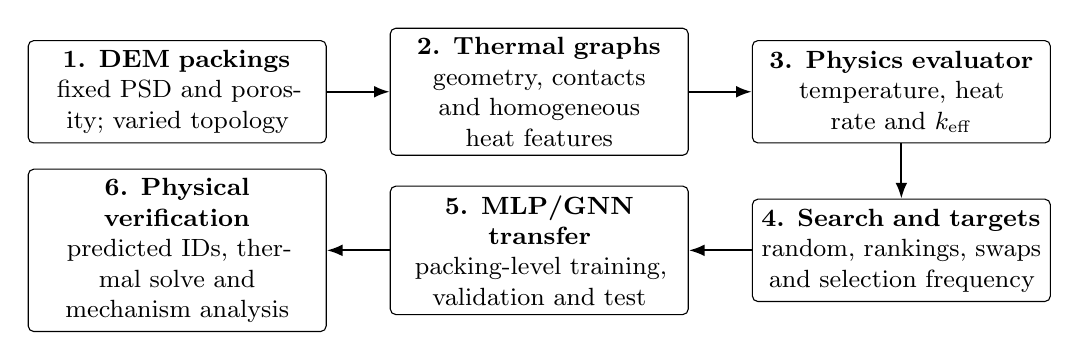
\begin{tikzpicture}[
			node distance=7mm and 8mm,
			box/.style={draw,rounded corners=2pt,align=center,minimum height=13mm,text width=3.55cm,font=\small},
			arrow/.style={-{Latex[length=2mm]},thick}
			]
			\node[box] (dem) {\textbf{1. DEM packings}\\fixed PSD and porosity; varied topology};
			\node[box, right=of dem] (graph) {\textbf{2. Thermal graphs}\\geometry, contacts and homogeneous heat features};
			\node[box, right=of graph] (solver) {\textbf{3. Physics evaluator}\\temperature, heat rate and $k_{\mathrm{eff}}$};
			\node[box, below=of solver] (alloc) {\textbf{4. Search and targets}\\random, rankings, swaps and selection frequency};
			\node[box, left=of alloc] (mechanism) {\textbf{5. MLP/GNN transfer}\\packing-level training, validation and test};
			\node[box, left=of mechanism] (validation) {\textbf{6. Physical verification}\\predicted IDs, thermal solve and mechanism analysis};
			\draw[arrow] (dem)--(graph);
			\draw[arrow] (graph)--(solver);
			\draw[arrow] (solver)--(alloc);
			\draw[arrow] (alloc)--(mechanism);
			\draw[arrow] (mechanism)--(validation);
		\end{tikzpicture}
		\caption{Computational workflow. DEM is run once per packing. The thermal
			network supplies physical baselines and search targets; MLP and GNN allocations
			are evaluated on complete unseen packings by the unchanged thermal solver.}
		\label{fig:workflow}
	\end{figure}
	
	\section{Results}
	
	\subsection{Homogeneous packing variability}
	
	With all particles assigned $k=1$~W\,m$^{-1}$\,K$^{-1}$, the ten packings gave
	\begin{equation}
		k_{\mathrm{eff,hom}}=0.09329\pm0.00351~\mathrm{W\,m^{-1}K^{-1}}.
	\end{equation}
	The range was 0.08615--0.09717~W\,m$^{-1}$\,K$^{-1}$ and the coefficient of
	variation was 3.77\%. The mean coordination number was
	$5.393\pm0.066$, with a smaller coefficient of variation of 1.22\%. Thus,
	packings with nearly identical contact counts still showed measurable thermal
	variation, indicating that contact arrangement and conductance weights matter.
	
	Between one and eleven particles per packing were outside the wall-anchored
	contact component. They carry no heat in the contact-only model and were
	excluded from the linear system. Every packing nevertheless contained one
	large component spanning both thermal walls.
	
	\subsection{Allocation performance across ten packings}
	
	Table~\ref{tab:summary} shows the ensemble results. Adding 10\% conductive
	particles at random raised the mean conductivity to
	$0.11046\pm0.00413$~W\,m$^{-1}$\,K$^{-1}$. Degree ranking produced only a small
	additional improvement and was slightly worse than the random mean in one
	packing. Heat-path ranking was better than random in all ten packings.
	
	\begin{table}[!htbp]
		\centering
		\caption{Performance across ten independent DEM packings. Improvement is
			calculated relative to the controlled random mean in the same packing.}
		\label{tab:summary}
		\small
		\begin{tabular}{P{4.1cm}P{3.7cm}P{3.7cm}}
			\toprule
			\textbf{Allocation} &
			$\boldsymbol{k_{\mathrm{eff}}}$ \textbf{[W/(m K)]} &
			\textbf{Mean improvement} \\
			\midrule
			Random mean & $0.11046\pm0.00413$ & reference \\
			Degree ranking & $0.11310\pm0.00425$ & $2.4\pm2.5$\% \\
			Heat-path ranking & $0.12208\pm0.00467$ & $10.5\pm2.3$\% \\
			Fixed-budget swap search, five-restart mean & $0.16868\pm0.00692$ & $52.7\pm3.5$\% \\
			Fixed-budget swap search, best of five & $0.17263\pm0.00787$ & $56.3\pm4.1$\% \\
			\bottomrule
		\end{tabular}
	\end{table}
	
	The best result from the five fixed-budget swap-search restarts improved on
	random placement in every realization.
	The smallest improvement was 50.8\% and the largest was 60.9\%. The mean
	improvement was 56.3\%, with a 95\% confidence interval of 53.4--59.2\%.
	The corresponding improvement over the homogeneous low-conductivity bed was
	$85.1\pm4.9$\%.
	
	\begin{table}[!htbp]
		\centering
		\caption{Per-packing controlled allocation results.}
		\label{tab:cases}
		\small
		\begin{tabular}{rrrrr}
			\toprule
			\textbf{Seed} & \textbf{Random mean} & \textbf{Heat path} &
			\textbf{Best swap search} & \textbf{Gain [\%]} \\
			\midrule
			18427 & 0.11123 & 0.12186 & 0.17895 & 60.9 \\
			29173 & 0.10194 & 0.11045 & 0.15600 & 53.0 \\
			37811 & 0.11317 & 0.12510 & 0.18102 & 60.0 \\
			46549 & 0.11216 & 0.12153 & 0.16918 & 50.8 \\
			55291 & 0.11330 & 0.12602 & 0.18219 & 60.8 \\
			64109 & 0.10562 & 0.12018 & 0.16895 & 60.0 \\
			72869 & 0.11075 & 0.12669 & 0.17540 & 58.4 \\
			81647 & 0.11472 & 0.12467 & 0.17498 & 52.5 \\
			90439 & 0.11402 & 0.12369 & 0.17334 & 52.0 \\
			99223 & 0.10774 & 0.12058 & 0.16628 & 54.3 \\
			\bottomrule
		\end{tabular}
	\end{table}
	
	The mean of the five final fixed-budget swap-search values was also substantially above
	random in every packing, with improvements between 48.7\% and 58.1\%. This
	shows that the conclusion does not depend only on selecting the best of five
	search trajectories.

	\subsection{Transfer to unseen packings with MLP and GNN}

	Table~\ref{tab:mlresults} reports the corrected three-repeat rank ensembles.
	Both learned models outperformed the transparent heat-path ranking in all ten
	held-out packings. The MLP reached
	$k_{\mathrm{eff}}=0.13137\pm0.00583$~W\,m$^{-1}$\,K$^{-1}$, corresponding to
	an improvement of $18.9\pm2.9$\% over random placement and recovery of
	$33.6\pm4.3$\% of the best-search gain. The edge-aware GNN reached
	$0.14189\pm0.00731$~W\,m$^{-1}$\,K$^{-1}$, or $28.4\pm3.8$\% above random, and
	recovered $50.7\pm7.7$\% of the searched gain. Its recovery fraction ranged
	from 41.9\% to 69.0\%.

	\begin{table}[!htbp]
		\centering
		\caption{Allocation performance on complete held-out packing graphs. Values
			are mean $\pm$ sample standard deviation over ten outer folds.}
		\label{tab:mlresults}
		\small
		\begin{tabular}{P{3.2cm}rrrr}
			\toprule
			\textbf{Method} & $\boldsymbol{k_{\mathrm{eff}}}$ & \textbf{vs. random} &
			\textbf{vs. heat path} & $\boldsymbol{f_{\mathrm{rec}}}$ \\
			& \textbf{[W/(m K)]} & \textbf{[\%]} & \textbf{[\%]} & \textbf{[\%]} \\
			\midrule
			Heat-path ranking & $0.12208\pm0.00467$ & $10.5\pm2.3$ & reference & --- \\
			Same-feature MLP & $0.13137\pm0.00583$ & $18.9\pm2.9$ & $7.6\pm1.9$ & $33.6\pm4.3$ \\
			Edge-aware GNN & $\mathbf{0.14189\pm0.00731}$ & $\mathbf{28.4\pm3.8}$ & $\mathbf{16.2\pm3.7}$ & $\mathbf{50.7\pm7.7}$ \\
			Fixed-budget swap search, best of five & $0.17263\pm0.00787$ & $56.3\pm4.1$ & --- & 100 \\
			\bottomrule
		\end{tabular}
	\end{table}

	The GNN exceeded the MLP in every held-out packing and increased mean effective
	conductivity by 8.0\% relative to the MLP. This is the central ablation result:
	because both models use identical node inputs, explicit contact and edge
	information provides useful predictive structure beyond particle-wise features.
	The result cannot be explained by splitting neighbouring particles between
	training and test data, because each test fold withholds the complete packing.

	\begin{table}[!htbp]
		\centering
		\caption{Fold-wise ensemble results. Recovery is defined by
			Eq.~\eqref{eq:recovered}.}
		\label{tab:mlfolds}
		\small
		\begin{tabular}{rrrrrr}
			\toprule
			\textbf{Fold} & \textbf{Test seed} & \textbf{MLP $k_{\mathrm{eff}}$} &
			\textbf{GNN $k_{\mathrm{eff}}$} & \textbf{MLP rec. [\%]} & \textbf{GNN rec. [\%]} \\
			\midrule
			1 & 18427 & 0.12987 & 0.13969 & 27.5 & 42.0 \\
			2 & 29173 & 0.11791 & 0.12849 & 29.5 & 49.1 \\
			3 & 37811 & 0.13781 & 0.14795 & 36.3 & 51.3 \\
			4 & 46549 & 0.12939 & 0.14353 & 30.2 & 55.0 \\
			5 & 55291 & 0.13445 & 0.14608 & 30.7 & 47.6 \\
			6 & 64109 & 0.13190 & 0.13665 & 41.5 & 49.0 \\
			7 & 72869 & 0.13377 & 0.14499 & 35.6 & 53.0 \\
			8 & 81647 & 0.13540 & 0.13994 & 34.3 & 41.9 \\
			9 & 90439 & 0.13636 & 0.15496 & 37.7 & 69.0 \\
			10 & 99223 & 0.12686 & 0.13665 & 32.7 & 49.4 \\
			\bottomrule
		\end{tabular}
	\end{table}

	Figure~\ref{fig:mlfolds} complements the numerical tables by showing whether the
	GNN advantage is consistent rather than produced by only one favourable packing.
	The GNN recovers more of the searched gain in every fold, although the magnitude
	varies with the contact topology.

	\begin{figure}[!htbp]
		\centering
		\IfFileExists{figures/gnn_loocv_recovered_gain.pdf}{%
			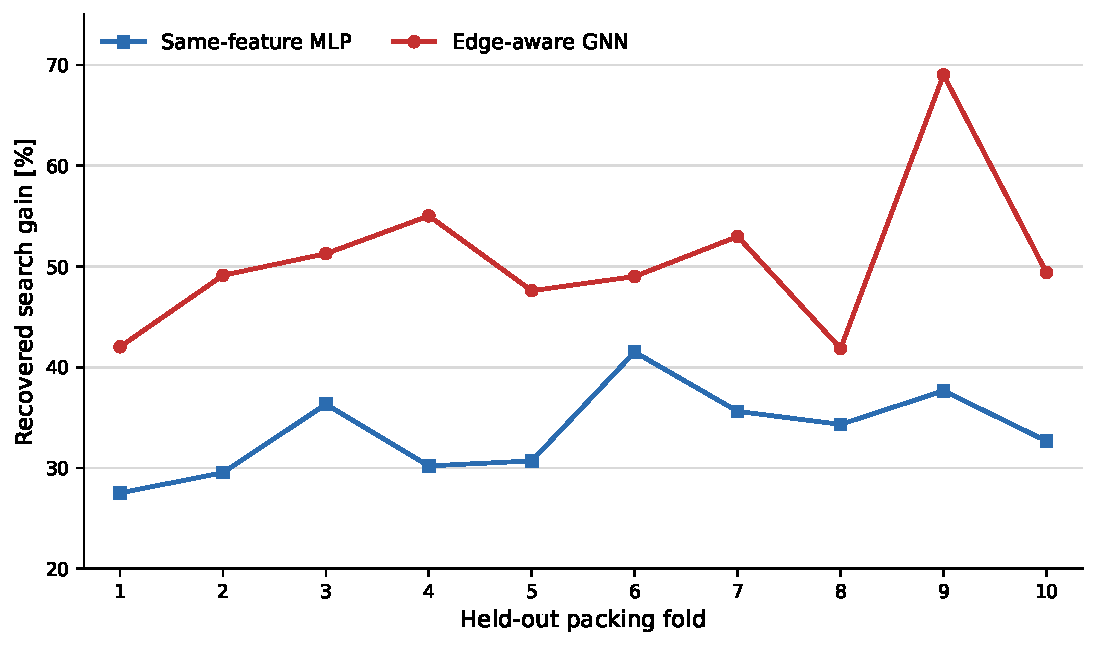
\includegraphics[width=0.86\textwidth]{figures/gnn_loocv_recovered_gain.pdf}%
		}{%
			\fbox{\parbox[c][6.2cm][c]{0.82\textwidth}{\centering
				Run \texttt{plot\_gnn\_loocv\_recovered\_gain.py} to generate\\
				\texttt{figures/gnn\_loocv\_recovered\_gain.pdf}}}%
		}
		\caption{Fraction of the best fixed-budget swap-search gain recovered on each
			held-out packing. The allocations are produced by three-repeat rank ensembles
			and evaluated by the unchanged thermal solver.}
		\label{fig:mlfolds}
	\end{figure}

	Mean Jaccard overlap with the single best searched ID set was 0.230 for the MLP
	and 0.254 for the GNN. These modest overlaps do not contradict the thermal
	improvement. The learning target combines five search restarts, and several
	different 50-particle assignments can reinforce alternative parallel pathways.
	Accordingly, thermally evaluated conductivity and recovered gain are the primary
	criteria; exact agreement with one stochastic teacher allocation is secondary.

\subsection{Computational cost}

The main purpose of the learned models is to avoid testing thousands of material
allocations on every new packing. Table~\ref{tab:cost} therefore compares the
work required to select and verify an allocation for one new packing.

Degree ranking requires one thermal-network solution to verify its selected
allocation. Heat-path ranking, the MLP and the GNN require two solutions: first,
the homogeneous bed is solved to obtain the baseline thermal information, and
then the selected allocation is solved to verify its effective conductivity.
The neural-network calculation between these two solutions is very fast.

The complete swap-search workflow is substantially more expensive. It includes
the random reference calculations, the degree and heat-path baselines, and five
search restarts with 3000 proposed swaps each. Across the ten packings, this
workflow required $14828.9\pm45.2$ distinct thermal-network solutions per
packing. Previously evaluated allocations were retrieved from a cache and were
not counted twice.

\begin{table}[!htbp]
	\centering
	\caption{Computational work required to select and verify an allocation for
		one new packing. Neural scoring time includes the three models used in the
		ensemble.}
	\label{tab:cost}
	\small
	\begin{tabular}{P{3.5cm}P{6.2cm}P{2.7cm}}
		\toprule
		\textbf{Method} &
		\textbf{Calculation performed} &
		\textbf{Thermal solves} \\
		\midrule
		Degree ranking &
		Count contacts, select particles and verify the allocation &
		1 \\
		
		Heat-path ranking &
		Solve the homogeneous bed, rank particles and verify the allocation &
		2 \\
		
		MLP ensemble &
		Solve the homogeneous bed, calculate particle scores and verify the
		allocation &
		2 \\
		
		GNN ensemble &
		Solve the homogeneous bed, calculate graph-based particle scores and
		verify the allocation &
		2 \\
		
		Full swap-search workflow &
		Evaluate random and ranked references and test allocations during five
		search restarts &
		$14828.9\pm45.2$ \\
		\bottomrule
	\end{tabular}
\end{table}

The three-model MLP and GNN ensembles required only
$(3.43\pm0.13)\times10^{-4}$~s and
$(3.96\pm0.13)\times10^{-3}$~s, respectively, to calculate the particle scores
on one packing. These CPU times are small compared with the thermal-network
solutions.

The models must first be trained using the previously generated search results.
Training the three models used in each ensemble required
$9.93\pm1.55$~s for the MLP and $30.70\pm9.19$~s for the GNN. This training is
performed once and is not repeated whenever the trained model is applied to
another packing.

Consequently, application of the trained GNN to a new packing requires two
thermal-network solutions and approximately 4~ms for graph-based particle
scoring. This replaces approximately 14829 trial solutions in the complete
swap-search workflow, corresponding to about 7400 times fewer thermal solves.
The GNN retained $50.7\pm7.7$\% of the conductivity gain found by that search.
	
	\subsection{Independent reproduction and conservation}
	
	The best ID list from every packing was independently evaluated by the thermal
	solver. All ten values reproduced the allocation-driver results exactly. Every
	independent calculation contained exactly 50 high-conductivity particles and
	the original DEM contact graph. The maximum relative difference between hot-
	and cold-side heat rates was $3.04\times10^{-12}$. These checks rule out output
	rounding, a changed graph or a mismatch in particle IDs as explanations for the
	observed improvement.
	
	\subsection{Mechanism comparison in a representative packing}
	
	To examine why the optimized assignment performs better, seed 18427 was
	analysed in greater detail. Three allocations were compared on exactly the same
	contact graph: a random realization closest to the random mean, heat-path
	ranking and the best result from the fixed-budget same-size swap search. The diagnostic quantities
	in Table~\ref{tab:mechanism} describe connections between high-conductivity
	particles, their contact with the thermal walls, and the heat carried by the
	resulting network.
	
	The indicators in Table~\ref{tab:mechanism} describe three complementary
	questions. First, how well is the conductive phase connected? The number of
	\emph{high--high contacts} counts direct contacts between two high-$k$ particles,
	while the number and size of \emph{high-$k$ clusters} show whether the 50 selected
	particles remain fragmented or form larger cooperative structures. A
	\emph{wall-spanning cluster} contains at least one particle touching each thermal
	wall; the separate hot/cold wall counts give the available heat-entry and
	heat-exit points.
	
	Second, are those connections useful for the imposed vertical heat flow? The
	\emph{high--high heat fraction} is the absolute contact heat carried by
	high--high contacts divided by that carried by all particle--particle contacts.
	The \emph{heat-weighted vertical alignment} averages $|\Delta z|/d_{ij}$ over
	high--high contacts using their absolute heat rates as weights; zero denotes a
	horizontal contact and one a vertical contact. Together, these measures
	distinguish active vertical pathways from conductive side branches.
	
	Third, what is the quality of the most favourable individual route? Assigning
	each link the resistance $1/G_{ij}$ gives the reported minimum-resistance
	hot-to-cold path, and the high-$k$ fraction states how much of that particle path
	is conductive. This series-path diagnostic is not the total bed resistance,
	because the complete network contains many parallel routes. The principal
	performance measure remains $k_{\mathrm{eff}}$, which combines all contacts and
	all pathways.
	
	\begin{table}[!htbp]
		\centering
		\caption{Mechanism comparison for packing seed 18427. The minimum-path
			resistance is a descriptive series-path indicator and not the total resistance
			of the parallel contact network.}
		\label{tab:mechanism}
		\small
		\begin{tabular}{P{5.1cm}rrr}
			\toprule
			\textbf{Indicator} & \textbf{Random} & \textbf{Heat path} & \textbf{Optimized} \\
			\midrule
			$k_{\mathrm{eff}}$ [W/(m K)] & 0.1112 & 0.1219 & \textbf{0.1789} \\
			High--high contacts & 17 & 27 & \textbf{55} \\
			Number of high-$k$ clusters & 35 & 26 & \textbf{5} \\
			Largest high-$k$ cluster [particles] & 6 & 5 & \textbf{26} \\
			Wall-spanning high-$k$ clusters & 0 & 0 & \textbf{2} \\
			High-$k$ particles linked to hot/cold wall & 4/2 & 0/0 & \textbf{7/6} \\
			Heat on high--high contacts [\%] & 4.6 & 9.1 & \textbf{41.3} \\
			Heat-weighted vertical alignment & 0.666 & 0.728 & \textbf{0.804} \\
			Minimum-path resistance [K/W] & 19894 & 15884 & \textbf{2892} \\
			High-$k$ fraction on minimum path [\%] & 63.6 & 55.6 & \textbf{100} \\
			\bottomrule
		\end{tabular}
	\end{table}

	\begin{figure}[!htbp]
		\centering
		\begin{minipage}[t]{0.24\textwidth}
			\centering
			\IfFileExists{figures/random.png}{%
				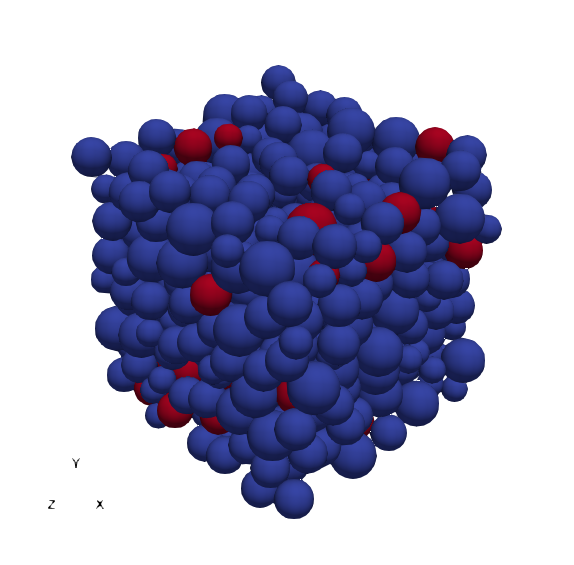
\includegraphics[width=0.7\linewidth,height=5.2cm,keepaspectratio]{figures/random.png}%
			}{\fbox{\parbox[c][5.0cm][c]{0.96\linewidth}{\centering
				Missing: \texttt{figures/random.png}}}}
			\\[-0.2em]\textbf{(a) Random near-mean allocation}
		\end{minipage}%\hfill
		\begin{minipage}[t]{0.24\textwidth}
			\centering
			\IfFileExists{figures/heatpath.png}{%
				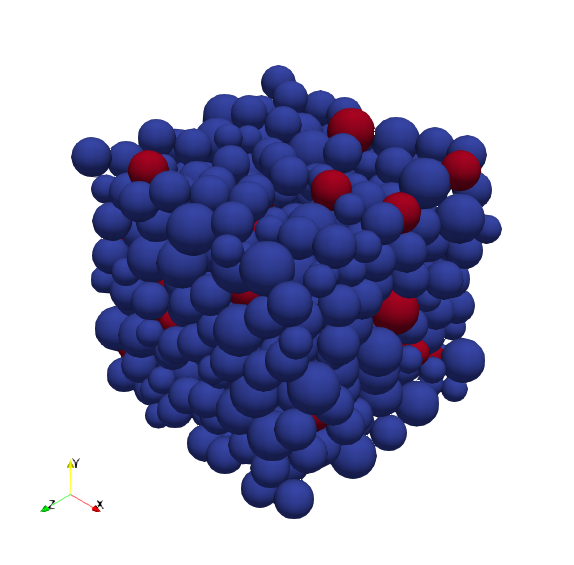
\includegraphics[width=0.7\linewidth,height=5.2cm,keepaspectratio]{figures/heatpath.png}%
			}{\fbox{\parbox[c][5.0cm][c]{0.96\linewidth}{\centering
				Missing: \texttt{figures/heatpath.png}}}}
			\\[-0.2em]\textbf{(b) Heat-path ranking}
		\end{minipage}
%		\vspace{0.8em}
		\begin{minipage}[t]{0.24\textwidth}
			\centering
			\IfFileExists{figures/gnn.png}{%
				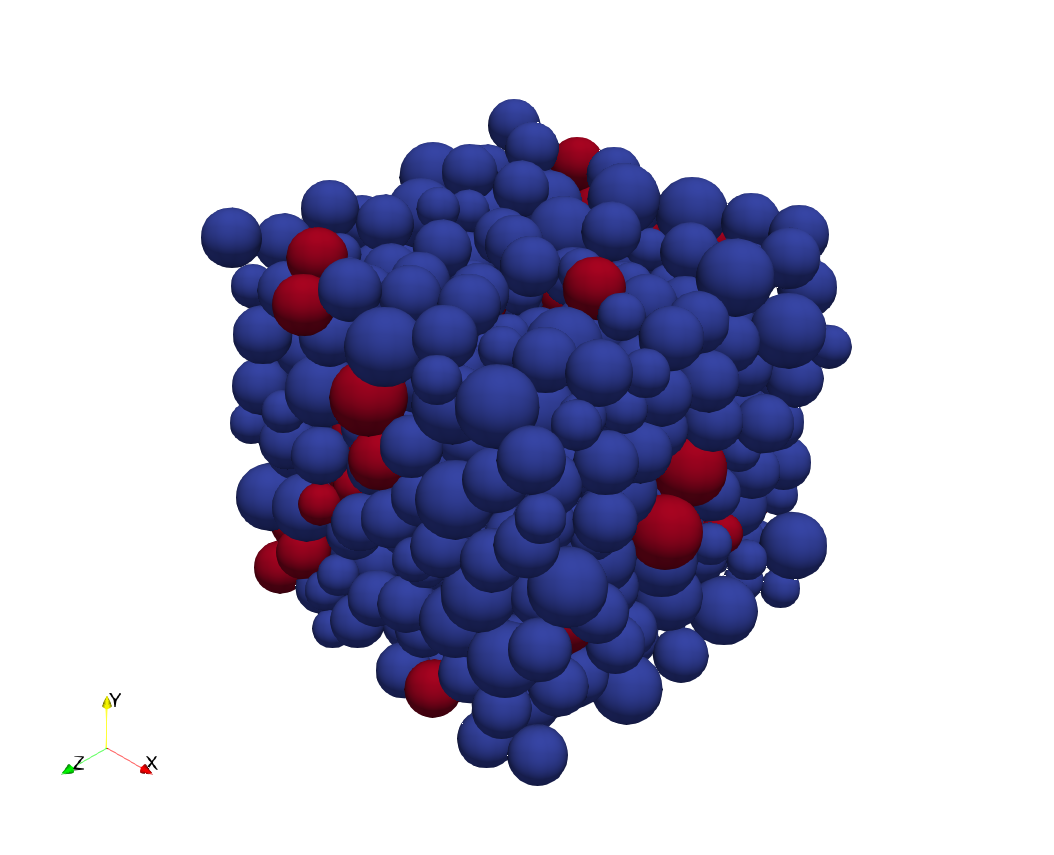
\includegraphics[width=0.85\linewidth,height=5.2cm,keepaspectratio]{figures/gnn.png}%
			}{\fbox{\parbox[c][5.0cm][c]{0.96\linewidth}{\centering
				Missing: \texttt{figures/gnn.png}}}}
			\\[-0.2em]\textbf{(c) Held-out GNN allocation}
		\end{minipage}%\hfill
		\begin{minipage}[t]{0.24\textwidth}
			\centering
			\IfFileExists{figures/swap.png}{%
				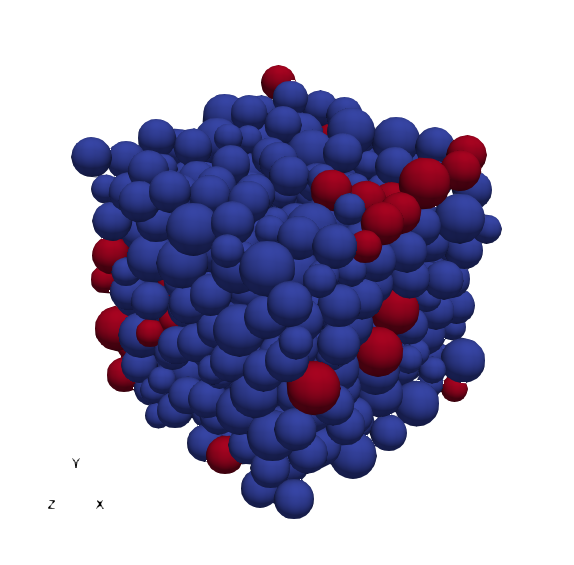
\includegraphics[width=0.7\linewidth,height=5.2cm,keepaspectratio]{figures/swap.png}%
			}{\fbox{\parbox[c][5.0cm][c]{0.96\linewidth}{\centering
				Missing: \texttt{figures/swap.png}}}}
			\\[-0.2em]\textbf{(d) Best swap-search allocation}
		\end{minipage}
		\caption{Comparison of four material allocations on packing seed
			18427: (a) a random realization closest to the random mean, (b) heat-path
			ranking, (c) the GNN rank ensemble obtained when this packing was held out,
			and (d) the best result from the fixed-budget same-size swap search.}
		\label{fig:paraview_allocations}
	\end{figure}
	
	The random allocation divided the 50 conductive particles into 35 mostly small
	clusters, and no all-conductive cluster connected the two walls. Heat-path
	ranking increased the number and vertical alignment of high--high contacts, but
		it also produced no wall-spanning conductive cluster. In contrast, the
	fixed-budget same-size swap search consolidated the conductive phase into five
	clusters. The largest
	contained 26 particles and two clusters connected the hot and cold boundaries.
	
	This structural change also altered where heat travelled. The fraction of the
	absolute particle-contact heat rate carried by high--high contacts increased
	from 4.6\% for the representative random allocation to 41.3\% after
	optimization. The heat-weighted vertical alignment of those contacts increased
	from 0.666 to 0.804. Moreover, all nine particles on the calculated
	minimum-resistance series path were conductive, and its resistance was 85.5\%
	lower than for the random allocation. These observations support a concrete
	mechanism: the optimizer forms several vertically useful, wall-connected
	conductive routes and reinforces the pre-existing heat-carrying backbone. The
	mechanism analysis currently concerns one representative packing and must be
	repeated for the complete ensemble before it is treated as a general result.
	
	\section{Discussion}
	
	The main result is simple: the same amount of conductive material can perform
	very differently depending on its position in the contact network. The weak
	performance of degree ranking explains why a purely local rule is insufficient.
	A particle may have many neighbours but still lie in a region with little net
	vertical heat flow. Heat-path ranking uses the direction and magnitude of the
	baseline heat flow and therefore performs better. Its consistent 8.3--14.4\%
	improvement is already a useful transparent result.
	
	The much larger gain from the fixed-budget swap search shows that conductive particles must
	be selected cooperatively. Changing one particle modifies the temperature and
	heat-flow distribution, which changes the usefulness of other particles. The
	representative mechanism comparison makes this interpretation more specific:
	the optimized assignment created two wall-spanning conductive clusters,
	strongly increased the heat carried by high--high contacts and produced a fully
	conductive minimum-resistance path. The design problem is therefore global:
	good assignments build several low-resistance routes between the thermal walls
	while avoiding isolated conductive clusters and redundant side branches.
	
	The study differs from a conventional conductivity-prediction exercise. The
	thermal equations remain the evaluator and the goal is to change a discrete
	material assignment under a strict budget. It also differs from inverse design
	of freely generated lattices \cite{Dold2023}: the contact topology here is
	mechanically produced by DEM and remains fixed during allocation.

	The ML comparison answers why a GNN is useful here. The MLP already performs
	better than heat-path ranking because its node features combine size, height,
	wall access, local degree and baseline thermal information. Nevertheless, it
	cannot represent how two candidate particles cooperate through their contacts.
	The GNN improves on the same-feature MLP in every held-out packing and recovers
	about half of the searched gain. Thus, graph learning is not introduced merely
	to predict a scalar bed property: it supplies a fast, quota-constrained material
	allocation that is checked by the governing thermal equations. Recovery below
	100\% is expected because the GNN performs a single forward ranking, whereas the
	teacher uses thousands of allocation proposals and repeated full-network solves.
	The result supports retaining the GNN while also retaining the transparent MLP,
	heat-path and search references.
	
	Several limitations define the present scope. First, the contact conductance
	uses a Hertzian radius derived from DEM overlap, so stiffness and packing
	pressure can affect the predicted magnitude. Second, the bed contains no
	validated fluid-phase conduction, convection or radiation. Third, only one
	conductive fraction and one conductivity contrast have been studied. Fourth,
	the ten independent graphs establish transfer across stochastic realizations of
	the defined 500-particle system, but not extrapolation to different PSDs,
	porosities, particle counts or boundary conditions. Finally, the fixed-budget
	swap search is stochastic; the reported assignments are the best found, not proven global
	optima. The GNN accordingly learns high-performing searched allocations rather
	than mathematically certified optima.
	
	\section{Conclusions}
	
	Ten equal-porosity, equal-PSD DEM packings were used to isolate the influence
	of conductive-particle placement. With an identical 10/30/10 size-class budget,
	degree ranking improved effective conductivity only slightly, while heat-path
	ranking gave a consistent mean improvement of 10.5\% over random placement.
	The best result from five fixed-budget swap-search restarts improved conductivity by 50.8--60.9\% in
	all ten packings. The effect therefore survives changes in random packing
	topology and cannot be attributed to conductive volume or particle-size bias.
	Exact independent reproduction and near-machine-precision energy conservation
	support the numerical reliability of the result. In the representative packing,
	optimization also produced two wall-spanning conductive clusters and increased
	the high--high contact heat fraction from 4.6\% to 41.3\%. This provides initial
	evidence that the improvement results from connected, vertically useful
	conductive pathways rather than from high local coordination alone.

	The packing-level ML experiment further establishes that the allocation rule is
	transferable. The same-feature MLP improved $k_{\mathrm{eff}}$ by 18.9\% over
	random placement and recovered 33.6\% of the best-search gain. The edge-aware
	GNN improved it by 28.4\%, recovered 50.7\% of the searched gain and exceeded
	both the MLP and heat-path rule in every one of the ten held-out packings. The
	comparison isolates the benefit of message passing because the two learned
	models use identical node features, training folds, loss, optimizer, stopping
	criterion, material quotas and thermal evaluator. For the investigated fixed
	packing specification, graph connectivity therefore contributes useful
	allocation information that cannot be reduced to independent particle scoring.
	
%	\section{Focused next steps}
%	
%	The numerical study and packing-level ML comparison are complete for the stated
%	scope. To keep the remaining work focused before submission, the next actions
%	should be limited to the following sequence.
%	
%	\begin{enumerate}
%		\item \textbf{Prepare the final figures and reproducibility archive.} Add a
%		fold-wise comparison plot for heat path, MLP, GNN and search; retain all DEM
%		inputs, packing summaries, allocation IDs, training outputs and random seeds.
%		
%		\item \textbf{Perform one targeted contact sensitivity check.} Repeat a small
%		subset using a changed elastic modulus or a normalized contact-resistance law.
%		The required result is stability of the method ranking, not equality of the
%		absolute conductivity. This directly addresses the softened DEM stiffness.
%		
%		\item \textbf{Finalize and submit within the present scope.} The ten-packing
%		leave-one-packing-out study is treated as the final dataset for transfer among
%		realizations of the specified bed. Additional packings or new PSD, porosity and
%		material conditions should be added only as a deliberate extension or if peer
%		review identifies statistical scope as a decisive concern. The separate
%		stagnant-fluid/pore-network extension can then be developed without delaying
%		the present contact-dominated paper.
%	\end{enumerate}
%	
	\begin{thebibliography}{99}

		\bibitem{CundallStrack1979}
		P.~A. Cundall and O.~D.~L. Strack,
		``A discrete numerical model for granular assemblies,''
		\emph{G\'{e}otechnique}, vol.~29, no.~1, pp.~47--65, 1979.
		\href{https://doi.org/10.1680/geot.1979.29.1.47}
		{doi:10.1680/geot.1979.29.1.47}.

		\bibitem{Zeng2025}
		G. Zeng, S. Hou, Q. Guo, Y. Cai and M. Xu,
		``Advances in solid particle thermal energy storage: A comprehensive review,''
		\emph{Sustainability}, vol.~17, no.~16, 7244, 2025.
		\href{https://doi.org/10.3390/su17167244}
		{doi:10.3390/su17167244}.

		\bibitem{Knoedler2019}
		P. Kn\"odler,
		``Thermo-mechanical investigations of packed beds for high temperature heat
		storage: Uniaxial compression test experiments and particle discrete
		simulations,''
		\emph{Applied Sciences}, vol.~9, no.~8, 1600, 2019.
		\href{https://doi.org/10.3390/app9081600}
		{doi:10.3390/app9081600}.

		\bibitem{Garitaonandia2024}
		E. Garitaonandia, P. Arribalzaga, I. Miguel and D. Bielsa,
		``Characterization of the ratcheting effect on the filler material of a steel
		slag-based thermal energy storage,''
		\emph{Energies}, vol.~17, no.~7, 1515, 2024.
		\href{https://doi.org/10.3390/en17071515}
		{doi:10.3390/en17071515}.

		\bibitem{Boribayeva2024}
		A. Boribayeva, X. Gvozdeva and B. Golman,
		``Packing characteristics and heat transfer performance of non-spherical
		particles for concentrated solar power applications,''
		\emph{Energies}, vol.~17, no.~18, 4552, 2024.
		\href{https://doi.org/10.3390/en17184552}
		{doi:10.3390/en17184552}.
		
		\bibitem{Batchelor1977}
		G.~K. Batchelor and R.~W. O'Brien,
		``Thermal or electrical conduction through a granular material,''
		\emph{Proceedings of the Royal Society of London A}, vol.~355,
		pp.~313--333, 1977.
		
		\bibitem{Vargas2001}
		W.~L. Vargas and J.~J. McCarthy,
		``Heat conduction in granular materials,''
		\emph{AIChE Journal}, vol.~47, no.~5, pp.~1052--1059, 2001.
		\href{https://doi.org/10.1002/aic.690470511}{doi:10.1002/aic.690470511}.
		
		\bibitem{Kiani2019}
		M. Kiani-Oshtorjani and P. Jalali,
		``Thermal discrete element method for transient heat conduction in granular
		packing under compressive forces,''
		\emph{International Journal of Heat and Mass Transfer}, vol.~145,
		118753, 2019.
		
		\bibitem{Joulin2020}
		C. Joulin, A. Xiang, P. D. Lee and C. E. Krill III,
		``Capturing heat transfer for complex-shaped multibody contact problems using
		the discrete element method,''
		\emph{Computational Particle Mechanics}, 2020.
		\href{https://doi.org/10.1007/s40571-020-00321-w}
		{doi:10.1007/s40571-020-00321-w}.
		
		\bibitem{Dold2023}
		D. Dold and D. Aranguren van Egmond,
		``Differentiable graph-structured models for inverse design of lattice
		materials,''
		\emph{Cell Reports Physical Science}, vol.~4, no.~10, 101586, 2023.
		\href{https://doi.org/10.1016/j.xcrp.2023.101586}
		{doi:10.1016/j.xcrp.2023.101586}.
		
		\bibitem{KernighanLin1970}
		B.~W. Kernighan and S. Lin,
		``An efficient heuristic procedure for partitioning graphs,''
		\emph{The Bell System Technical Journal}, vol.~49, no.~2,
		pp.~291--307, 1970.
		\href{https://doi.org/10.1002/j.1538-7305.1970.tb01770.x}
		{doi:10.1002/j.1538-7305.1970.tb01770.x}.
		
		\bibitem{Maringer2003}
		D. Maringer and H. Kellerer,
		``Optimization of cardinality constrained portfolios with a hybrid local
		search algorithm,''
		\emph{OR Spectrum}, vol.~25, pp.~481--495, 2003.
		\href{https://doi.org/10.1007/s00291-003-0139-1}
		{doi:10.1007/s00291-003-0139-1}.
		
		\bibitem{Battaglia2018}
		P.~W. Battaglia et al.,
		``Relational inductive biases, deep learning, and graph networks,''
		\emph{arXiv preprint arXiv:1806.01261}, 2018.
		\href{https://doi.org/10.48550/arXiv.1806.01261}
		{doi:10.48550/arXiv.1806.01261}.
		
		\bibitem{LAMMPSGranular}
		LAMMPS Developers,
		``\texttt{pair\_style granular} command,'' LAMMPS documentation.
		\href{https://docs.lammps.org/pair_granular.html}
		{docs.lammps.org/pair\_granular.html}.

		\bibitem{LAMMPSNVESphere}
		LAMMPS Developers,
		``\texttt{fix nve/sphere} command,'' LAMMPS documentation.
		\href{https://docs.lammps.org/fix_nve_sphere.html}
		{docs.lammps.org/fix\_nve\_sphere.html}.
		
	\end{thebibliography}
	
\end{document}
